% SpinVL -- single-file build for Overleaf.
% Figures are expected at project root or in figures/ (all four PNGs are uploaded).
\documentclass[10pt,twocolumn,letterpaper]{article}

\usepackage[letterpaper,text={6.875in,8.875in},centering,top=1in]{geometry}
\usepackage{times}
\usepackage{graphicx}
\usepackage{amsmath,amssymb}
\usepackage{booktabs}
\usepackage{multirow}
\usepackage{array}
\usepackage{xcolor}
\usepackage[font=small,labelfont=bf,textfont=small]{caption}
\usepackage[numbers,sort&compress]{natbib}
\usepackage[hidelinks]{hyperref}

\graphicspath{{figures/}{./}}
\setlength{\columnsep}{0.31in}
\renewcommand{\arraystretch}{1.05}

\newcommand{\modelname}{SpinVL}
\newcommand{\ie}{\emph{i.e.}}
\newcommand{\eg}{\emph{e.g.}}

\begin{document}

\twocolumn[{
\begin{center}
{\LARGE\bfseries \modelname: Turning Frozen Text LLMs into Vision-Language\\[2pt]
Models with Zero Visual Tokens in the Backbone\par}
\vspace{10pt}
{\large Anonymous CVPR submission\par}
\vspace{4pt}
{\small Paper ID 0000\par}
\end{center}
\vspace{6pt}
\begin{center}
\begin{minipage}{0.90\textwidth}
\small
\textbf{Abstract}
\vspace{3pt}

Vision-language models (VLMs) built by concatenating visual tokens into a
frozen or fine-tuned LLM pay a steep price: attention cost grows with image
resolution, and adapting the backbone erodes the language model's original
text reasoning. Parameter-rotation methods remove visual tokens from the
backbone, but still depend on a heavy external vision tower, and they
deteriorate once the model generates autoregressively on its own. We introduce
\modelname, a framework that converts a completely frozen pure-text LLM into a
VLM that keeps \textbf{zero visual tokens in the backbone} and, in its
strongest configuration, \textbf{removes the external vision tower entirely}.
\modelname{} rests on two mechanisms. A \emph{dual-tier orthogonal rotation}
architecture first repurposes the student's own first $K{=}4$ layers as a
built-in vision encoder through static Cayley rotation and channel-wise
scaling ($2.4$M parameters), then discards every image token and modulates the
deeper frozen layers with dynamic block-diagonal rotations generated by
multi-frequency or spatial-anchor queries. Because the text pathway is left
untouched, pure-text behaviour is bit-exact, whereas merging the same vision
adapters into the backbone collapses GSM8K from $70.4\%$ to $0.0\%$.
Second, \emph{online policy distillation} (VL-OPD) supervises the student's
own rollouts with token-level KL from a stronger VLM, which lifts free-form
generation by up to $+9.9$ points. With the same training data, steps, and
frozen base model, \modelname{} outperforms a token-concatenation LLaVA
baseline on visual perception and anti-hallucination
($44.37\%$ vs.\ $41.35\%$), matches it on the average of perception,
hallucination and mathematical reasoning ($35.90\%$ vs.\ $35.87\%$), is
strictly better than single-frequency rotation and LoRA-based built-in
encoders, and does so with $74.2\%$ fewer FLOPs and $100\%$ preserved text
ability.
\end{minipage}
\end{center}
\vspace{10pt}
}]

\section{Introduction}
\label{sec:intro}

\begin{figure*}[t]
\centering
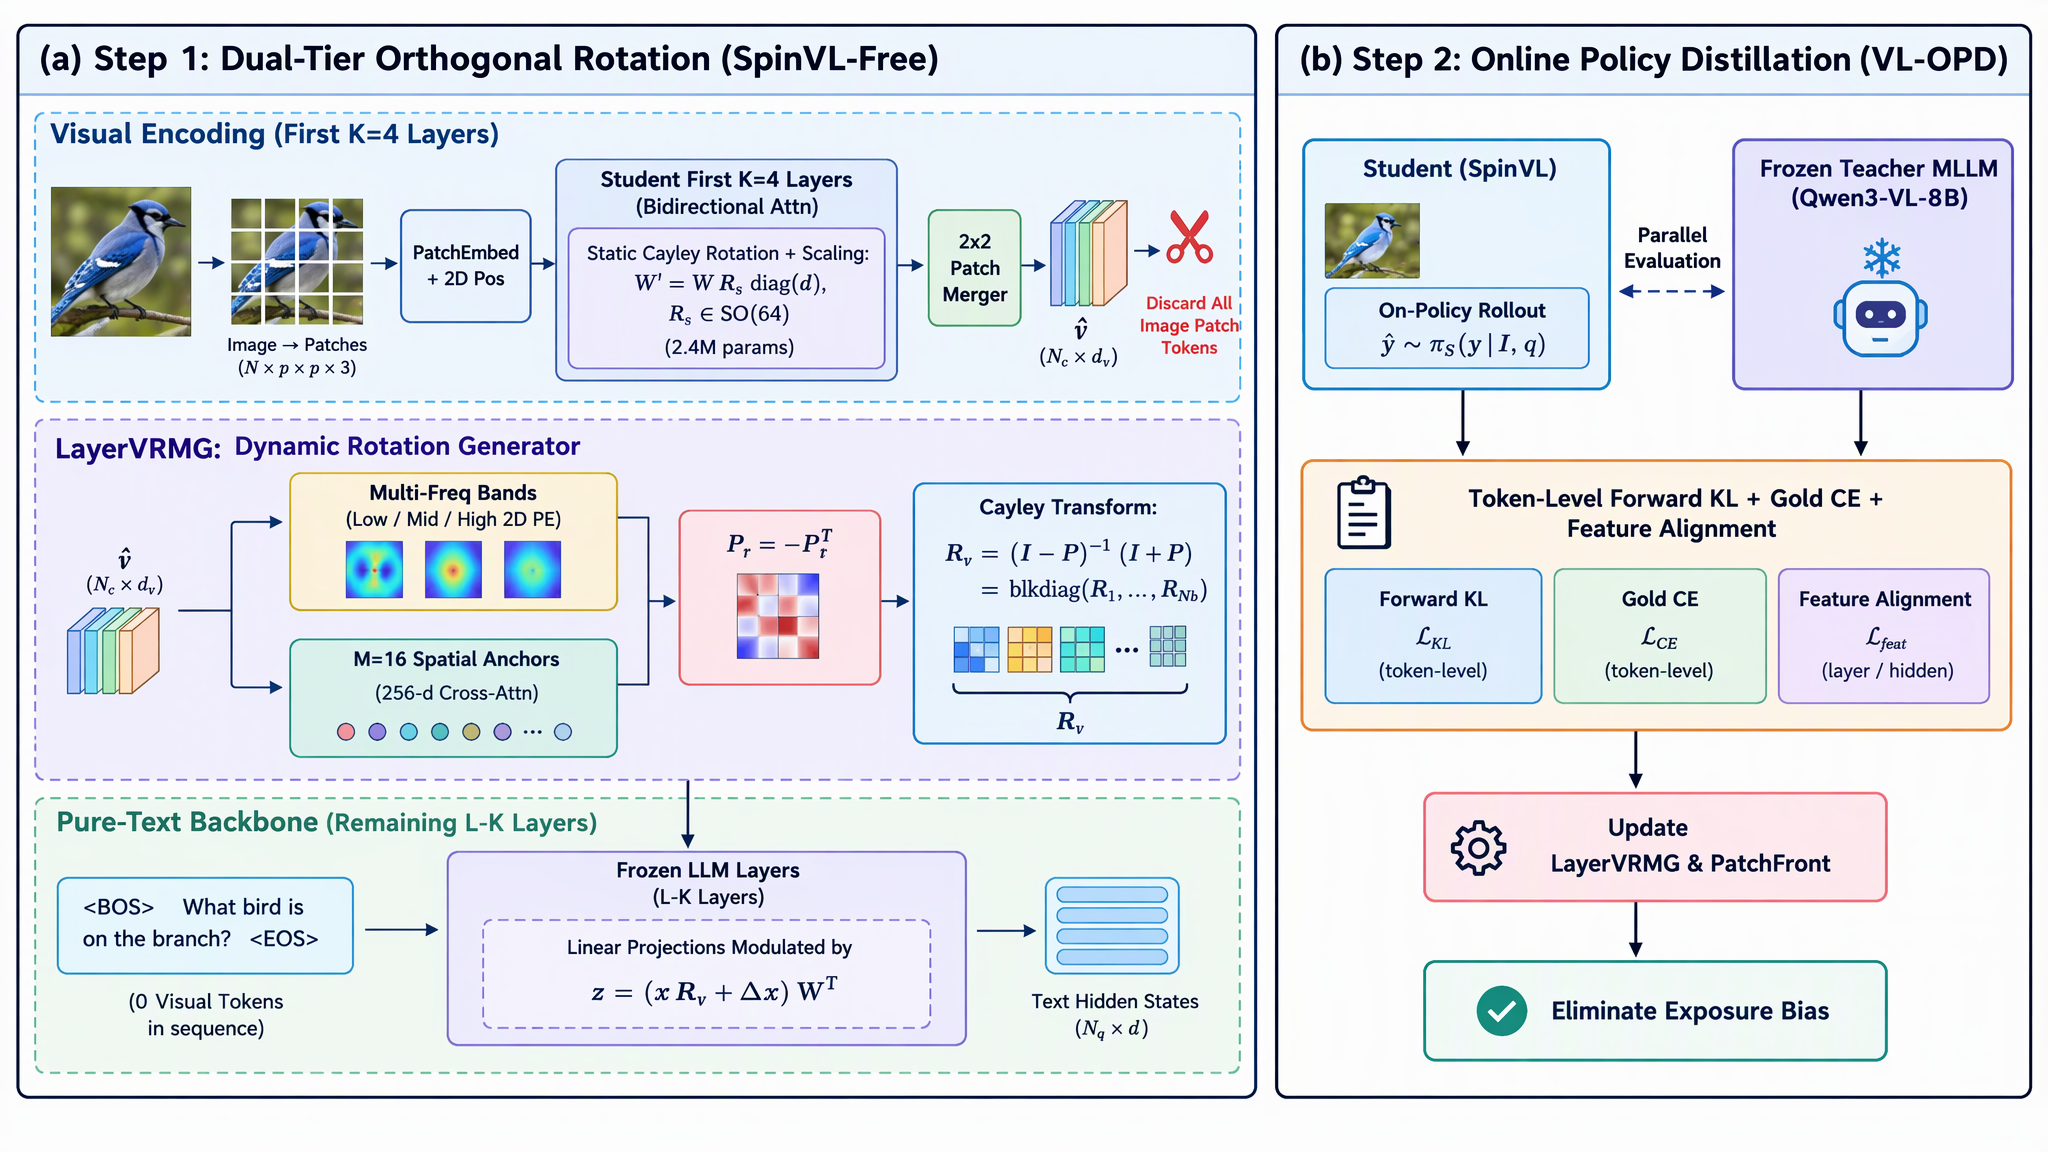
\includegraphics[width=0.98\textwidth]{fig_architecture.png}
\caption{\textbf{Overview of \modelname.} A completely frozen pure-text LLM is
turned into a VLM without any visual token inside the deeper backbone.
\emph{Step~1 (dual-tier orthogonal rotation):} the student's own first
$K{=}4$ layers act as a built-in vision encoder with static Cayley rotation
and channel scaling; all image tokens are discarded after layer $K$, and a
compact cell feature drives dynamic block-diagonal rotations in the remaining
layers. \emph{Step~2 (online policy distillation):} the student samples its
own trajectories and is supervised token-by-token by a stronger VLM, which
removes the exposure bias of teacher-forced training. The text pathway is
never modified, so pure-text behaviour is bit-exact.}
\label{fig:arch}
\end{figure*}

Feeding images to a language model is usually done by concatenation: a vision
encoder, often a full ViT with hundreds of millions of parameters, turns the
image into a sequence of tokens that is prepended to the text and propagated
through every layer of the LLM~\citep{liu2023llava,liu2024improved}. This
recipe is simple and effective, but it couples image resolution to the cost of
the language model. At $4096$ patches, a $1.7$B student with $28$ layers
spends $9.85$ TFLOPs per forward pass, an order of magnitude more than the
text-only model would; the KV cache grows with the same factor. The usual
remedy, fine-tuning the backbone on image-text pairs, trades away a property
that is expensive to recover: the instruction-following and mathematical
ability of the original model.

An appealing alternative is to modulate weights instead of extending the
context. Rotation-based injection~\citep{rose2025} keeps the backbone free of
visual tokens by mapping visual features to block-diagonal orthogonal matrices
that rotate the inputs of linear projections. It inherits the text model
untouched and removes the quadratic cost of long visual sequences. Three
problems remain. First, the method still requires an external vision tower,
which is exactly the component one would like to delete when deploying a
single frozen LLM. Second, images are pooled into one static rotation, so
spatial detail is lost and the model cannot revisit a region. Third, the
model is trained with teacher forcing on ground-truth answers; at inference
time it must consume its own prefixes, and small early errors compound---we
observe degenerate repetitions and missing end-of-sequence tokens.

A parallel line of work replaces the vision tower with the LLM's own early
layers~\citep{vora2025}. This removes the tower but keeps the visual tokens
alive: they travel through all remaining layers, so no compute is saved, and
merging the resulting low-rank adapters into the backbone destroys text
reasoning (GSM8K drops from $70.4\%$ to $0.0\%$ in our controlled experiment).

This paper asks whether one can have all three properties at once: no
external vision tower, no visual token in the deeper backbone, and intact text
ability. \modelname{} answers affirmatively with a two-step framework
(Fig.~\ref{fig:arch}).

\textbf{Step~1: dual-tier orthogonal rotation.} We distinguish two tiers of
adaptation. In the shallow tier, the student's first $K$ layers are
repurposed as a vision encoder using \emph{static} orthogonal rotation
combined with a channel-wise diagonal scaling, which preserves angular
geometry yet, unlike a pure rotation, can rescale singular values. Only
$2.4$M parameters are involved. After layer $K$ every image token is dropped
and a compact set of cell features remains. In the deep tier, those features
generate \emph{dynamic} block-diagonal rotations for the remaining frozen
layers. We propose two complementary generators: a multi-frequency variant
that splits rotation blocks into low-, mid-, and high-frequency bands with
RoPE-style positional encodings, and a hybrid variant that adds a lightweight
cross-attention over a handful of spatial anchors. The two target different
abilities---multi-step diagram reasoning versus fine-grained perception---and
we report both.

Because rotations are applied through a context-local wrapper, the text
pathway is untouched: with the vision branch switched off the model is
bit-identical to the original LLM ($70.4\%$ GSM8K, $71.4\%$ ARC-C). This is
not true for additive adapters or for permanently merged rotations, whose text
accuracy collapses.

\textbf{Step~2: online policy distillation.} Offline teacher forcing trains
the model only on ground-truth prefixes. We therefore let the student roll out
its own answers and ask a stronger VLM to score exactly those tokens with a
full-vocabulary forward KL, anchored by a gold cross-entropy term. Five
hundred steps suffice to raise free-form generation by $+4.1$ to $+9.9$
points across benchmarks and to bring end-of-sequence termination above
$95\%$.

\textbf{Controlled evidence.} All models in our main table share the same
frozen base model, the same training mixture, and the same optimisation
budget; the token-concatenation baseline is retrained by us rather than quoted.
Under this protocol \modelname{} improves the average of perception and
anti-hallucination from $41.35\%$ to $44.37\%$ without any visual token in the
backbone, reaches $35.90\%$ on the average of perception, hallucination and
mathematical reasoning against $35.87\%$ for the token-concatenation
baseline, and, in the tower-free configuration, retains $97.4\%$ of that
baseline's score while using $74.2\%$ fewer FLOPs and running $19.5\%$ faster
at high resolution.

Finally, we characterise the limits of the paradigm instead of hiding them.
By re-training the concatenation baseline on identical data that includes
open-ended chart and document questions, we show that its accuracy on
character-level chart reading and OCR stays flat ($10.32\%$ and $1.10\%$),
while our model stays in the low single digits; adding the same data doubles
our geometry accuracy. Operator-level modulation therefore buys semantic
perception, hallucination resistance and diagram reasoning, but not dense
transcription, which appears to require per-position key-value addressing.

Our contributions are:
\begin{itemize}
\item A dual-tier orthogonal rotation architecture that keeps zero visual
tokens in the backbone and needs no external vision tower, using $2.4$M
static parameters to turn the student's first layers into a vision encoder and
discarding all image tokens thereafter.
\item Multi-frequency and spatial-anchor rotation generators for the deep
tier, together with a modality-decoupled wrapper that makes pure-text
behaviour bit-exact.
\item An online policy distillation stage that repairs autoregressive drift of
rotation-injected models with $500$ steps of on-policy token-level KL.
\item A controlled study against token concatenation, single-frequency
rotation and LoRA-based built-in encoders, covering $0.6$B--$8$B students,
three seeds, compute, latency, text retention, and an explicit statement of
the paradigm's operating envelope.
\end{itemize}

\section{Related Work}
\label{sec:related}

\paragraph{Token-concatenation VLMs.}
LLaVA-style models connect a pretrained vision encoder to an LLM through a
light projector and train on instruction data~\citep{liu2023llava,
liu2024improved}. Scaling this recipe mostly means scaling the visual token
count, which is precisely what makes inference expensive at high resolution.
Our baseline belongs to this family and is retrained under our data and
compute budget so that comparisons are apples-to-apples.

\paragraph{Parameter-efficient adaptation.}
Low-rank adapters~\citep{hu2021lora} insert trainable matrices next to frozen
weights. VoRA-style built-in encoders~\citep{vora2025} apply them to the
LLM's early layers and distil a vision tower, thereby removing the tower but
keeping visual tokens in the sequence. Additive adapters also perturb the
weights permanently; our measurements show that merging them into a text model
destroys arithmetic reasoning, which motivates a multiplicative,
context-gated form of adaptation.

\paragraph{Rotation-based injection.}
ROSE~\citep{rose2025} converts visual features into block-diagonal orthogonal
matrices and rotates linear inputs, so the backbone never sees a visual token.
The construction guarantees that activations preserve their norm, and it is
attractive because the text model remains intact. Its limitations---a static,
globally pooled rotation, dependence on an external tower, and exposure bias
under greedy decoding---are the starting point of this work. We keep the
orthogonal construction, make it dynamic and spatially addressable, remove the
tower, and add on-policy distillation.

\paragraph{Distillation for VLMs.}
Knowledge distillation transfers a teacher's output distribution to a
student~\citep{hinton2015distilling}; sequence-level variants have been used
to compress captioning and VQA models. Off-policy distillation on
ground-truth prefixes, however, does not cover the states a model visits when
it decodes on its own. Online policy distillation---sampling from the student
and scoring those samples---closes this gap and is the second step of our
framework.

\paragraph{Orthogonal parameterisation.}
The Cayley transform $R=(I-A)^{-1}(I+A)$ maps a skew-symmetric matrix to a
special orthogonal matrix~\citep{golub2013matrix} and has been used to
stabilise recurrent and convolutional models. We use it to parameterise
block-diagonal rotations that are cheap to generate, exactly orthogonal, and
composable with a learned diagonal rescaling.

\paragraph{Benchmarks.}
We evaluate on general perception (MMStar~\citep{chen2024mmstar}), visual
hallucination (HallusionBench~\citep{guan2024hallusionbench}), chart reasoning
(ChartQA~\citep{masry2022chartqa}), scene-text understanding
(OCRBench~\citep{liu2023ocrbench}), mathematical reasoning
(MathVista~\citep{lu2024mathvista}), and plane geometry
(Geometry3K~\citep{lu2021geometry3k}). Text retention is measured with GSM8K
\citep{cobbe2021gsm8k} and ARC-Challenge~\citep{clark2018arc}.

\section{Method}
\label{sec:method}

\subsection{Overview and Notation}
\label{sec:overview}

Let $f_\theta$ be a frozen pure-text LLM with $L$ layers and hidden width
$d$, and let $\mathcal{S}\subset\{1,\dots,L\}$ be the set of layers we
modulate. An image is processed into $N$ patches by the teacher's image
processor. \modelname{} never places those patches inside the context of the
deeper layers. Instead, it produces a compact set of cell features
$V\in\mathbb{R}^{N_c\times d_v}$ and uses them to rotate the inputs of the
seven linear projections ($q,k,v,o,\text{gate},\text{up},\text{down}$) in
layers $\mathcal{S}$, as illustrated in Fig.~\ref{fig:arch}.

Two model variants share this skeleton. \emph{\modelname-Tower} takes $V$
from a frozen external vision encoder and is the direct successor of
rotation-based injection. \emph{\modelname-Free} additionally deletes the
encoder: $V=\hat{v}$ is produced by the student's own first $K$ layers, and
all image tokens are dropped afterwards. Both variants are followed by the
same on-policy distillation stage.

\subsection{Tier 1: Built-in Vision Frontend}
\label{sec:frontend}

\paragraph{Static rotation with channel scaling.}
A pure orthogonal rotation preserves norms and angles but cannot change
singular values, so it can re-aim features without re-weighting channels. We
therefore compose a rotation with a learned diagonal rescaling,
\begin{equation}
W' = W\,R_{\mathrm{s}}\,\mathrm{diag}(d),
\qquad
R_{\mathrm{s}} = (I-A)^{-1}(I+A),
\label{eq:static}
\end{equation}
where $A$ is skew-symmetric, $R_{\mathrm{s}}\in SO(b)$ acts on $b{=}64$
channel blocks, and $d\in\mathbb{R}^{d_{\text{in}}}$ is initialised to ones.
Because $R_{\mathrm{s}}$ is orthogonal, training stays well conditioned and
the rescaling supplies the degrees of freedom that orthogonality removes. For
$K{=}4$ layers and seven projections this amounts to $2.4$M parameters,
compared with $201$M for copying the layers and $3.7$M for rank-$16$ LoRA.

\paragraph{Reading the image once.}
Image patches are linearly embedded and given row and column positional
embeddings. They are then propagated through the student's first $K$ layers
with \emph{bidirectional} attention under Eq.~\eqref{eq:static}, which lets
every patch see the whole image---the regime a vision encoder needs and the
regime a causal LLM never provides. Adjacent $2\times2$ patches are
concatenated and projected by a two-layer merger into one cell feature,
\begin{equation}
\hat{v} = \mathrm{MLP}\big(\mathrm{LN}([h_{4i},h_{4i+1},h_{4i+2},h_{4i+3}])\big)
\in\mathbb{R}^{d_v},
\label{eq:merge}
\end{equation}
yielding $\hat{v}\in\mathbb{R}^{N_c\times d_v}$ with $N_c=N/4$.

\paragraph{Discard, then modulate.}
After Eq.~\eqref{eq:merge} the image tokens are deleted: the remaining
$L-K$ layers see a purely textual sequence. The only trace of the image is
$\hat{v}$, which drives the deep rotations of Sec.~\ref{sec:dynamic}. This is
the structural difference from built-in-encoder approaches that keep the
patches in the sequence.

\paragraph{Optional feature supervision.}
When a teacher encoder is available during training we align $\hat{v}$ with
its cell features $v^{\ast}$ through
\begin{equation}
\mathcal{L}_{\mathrm{feat}} = \frac{1}{N_c}\sum_{i}\Big[(1-\cos(\hat v_i,v^\ast_i))
+ \lambda_1\,\ell_{\mathrm{smooth}}\big(\tfrac{\hat v_i}{s},\tfrac{v^\ast_i}{s}\big)\Big],
\label{eq:feat}
\end{equation}
with $s=\mathrm{std}(v^\ast)$ and $\lambda_1{=}0.5$. This term only shapes the
frontend during training; it is not needed at inference and, as we show in
Sec.~\ref{sec:abl}, the model still learns to read images when it is
switched off entirely.

\subsection{Tier 2: Dynamic Rotation Injection}
\label{sec:dynamic}

\paragraph{Generating a rotation per layer.}
For a layer $\ell\in\mathcal{S}$ we keep $N_b$ learnable queries
$Q_\ell\in\mathbb{R}^{N_b\times d_q}$ ($d_q{=}256$). Visual features are
projected to keys and values, and the queries read out a context
\begin{equation}
C_\ell = \mathrm{MHA}\big(Q_\ell,\; W_k^{(\ell)}V,\; W_v^{(\ell)}V\big),
\qquad
\theta_\ell = W_o^{(\ell)}C_\ell ,
\label{eq:ctx}
\end{equation}
where $\theta_\ell\in\mathbb{R}^{N_b\times b(b-1)/2}$ collects the strictly
lower-triangular entries of the skew-symmetric blocks. The rotation is
\begin{equation}
A_r = \mathrm{tril}(\theta_{\ell,r}) - \mathrm{tril}(\theta_{\ell,r})^{\top},
\qquad
R_{\ell,r} = (I-A_r)^{-1}(I+A_r),
\label{eq:cayley}
\end{equation}
and a rotated projection computes
\begin{equation}
y = \big(x\,R_{\ell}\big)W^{\top}+b,
\qquad
R_\ell = \mathrm{blkdiag}(R_{\ell,1},\dots,R_{\ell,N_b}),
\label{eq:rotlin}
\end{equation}
with $x$ split into $N_b$ channel blocks. All seven projections of a layer
share the same visual context, which is computed once and cached for the whole
forward pass, so generation pays for the rotation generator once per layer
rather than once per step.

\paragraph{Multi-frequency rotation (\texttt{mf}).}
A single pooled context forces every block to look at the image through the
same aperture. We split the $N_b$ blocks into three bands, following the
frequency division of rotary position embeddings~\citep{su2024roformer}. 
Low-frequency blocks attend to the globally pooled feature $\bar v$;
mid-frequency blocks
attend to all cells with a smooth positional encoding
($\mathrm{base}{=}10^4$); high-frequency blocks use a rapidly varying encoding
($\mathrm{base}{=}50$, softmax temperature $\tau{=}0.25$) to sharpen
localisation. A zero-initialised gate then mixes rotation with identity,
\begin{equation}
\tilde x_r = x_r + 2\sigma\big(W_g x\big)_r\,\big(x_rR_{\ell,r}-x_r\big),
\label{eq:gate}
\end{equation}
so the model starts from the pretrained function and adds rotation only where
it helps. This variant favours multi-step reasoning over diagrams, where the
model must repeatedly consult a small region.

\paragraph{Spatial-anchor hybrid (\texttt{hyb}).}
The second variant keeps the orthogonal rotation and adds a residual that can
address a few locations,
\begin{equation}
\Delta x = W_{\mathrm{out}}\,
\mathrm{MHA}\big(W_q\,\mathrm{LN}(x),\, K_a,\, V_a\big),
\qquad
y=\big(xR_\ell+\Delta x\big)W^{\top}+b,
\label{eq:hyb}
\end{equation}
where $K_a,V_a$ come from $M{=}16$ learnable anchors pooled from $V$, and
$W_{\mathrm{out}}$ is zero-initialised. The cross-attention lives in the
$d_q$-dimensional subspace, so it costs $O(TM d_q)$ instead of
$O(TN d)$; no visual token enters self-attention. This variant favours
perception and hallucination tests, where a single global transform is too
coarse to decide whether a small object is present.

Both variants are single switches; the backbone stays frozen in all cases.

\subsection{Modality Decoupling}
\label{sec:decouple}

The rotations act through a context-local wrapper that is active only inside
the image branch. When no visual context is set, each wrapped projection calls
its original weight, so a text-only input follows exactly the computation of
the unmodified LLM and produces bit-identical logits. This is what allows
\modelname{} to claim lossless text ability while still being trained on image
data. It also explains a negative result we report in
Sec.~\ref{sec:eff}: any variant that merges vision adapters into the text
pathway---LoRA, static rotation, or rotation with scaling---loses most of its
arithmetic ability, which is why the decoupled design is not a convenience but
a requirement.

\subsection{Step 2: Online Policy Distillation}
\label{sec:opd}

Teacher-forced training only visits prefixes of ground-truth answers. Greedy
decoding visits the student's own prefixes, where a small early error moves
the hidden state off the training manifold; rotation-injected models are
particularly sensitive because the rotation is conditioned on the current
hidden state itself. We therefore distil on-policy.

Let $\hat y_{1:T}\sim\pi_S(\cdot\mid I,q)$ be a rollout sampled from the
student with the vision context active. A frozen teacher VLM
$\pi_T$ (an instruction-tuned model of the same tokenizer family) scores the
\emph{same} trajectory in one forward pass, giving
\begin{equation}
\mathcal{L}_{\mathrm{OPD}}=
\mathbb{E}_{\hat y}\Big[\sum_{t=1}^{T}
\mathrm{KL}\!\left(\pi_T(\cdot\mid I,q,\hat y_{<t})\,\Big\|\,
\pi_S(\cdot\mid I,q,\hat y_{<t})\right)
+\lambda_{\mathrm{ce}}\,\mathcal{L}_{\mathrm{CE}}\Big],
\label{eq:opd}
\end{equation}
where the cross-entropy term anchors the model to gold tokens that appear in
the rollout. For \modelname-Free{} we add Eq.~\eqref{eq:feat} with a small
weight to keep $\hat v$ stable while the frontend is updated. Training uses
$500$ steps, batch size $4$, learning rates $2\times10^{-5}$ (rotation) and
$10^{-5}$ (frontend), and takes under fifteen minutes on one GPU. The
distillation is thus a cheap post-hoc stage rather than a second training run.

\subsection{Complexity}
\label{sec:complexity}

For a text length $T$ and $N$ visual patches, a token-concatenation layer
attends over $T+N$ positions, costing $O((T+N)^2d)$; the visual part alone is
$O(2TNd+N^2d)$ and is paid in every layer. \modelname{} pays $O(N^2d)$ for
$K$ early layers in the frontend and, in the remaining $L-K$ layers, only
$O(T^2d)$ for self-attention plus $O(TN d_q)$ for the anchor residual, with
$d_q\ll d$. The block rotations add $O(Tdb)$, independent of both $N$ and the
number of projections' output width in the leading term. Measured at $4096$
patches the total drops from $9.85$ to $2.54$ TFLOPs
(Tab.~\ref{tab:eff}), and because the frontend encodes patches once with
bidirectional attention, wall-clock latency at high resolution improves as
well.

\section{Experiments}
\label{sec:exp}

\subsection{Setup}
\label{sec:setup}

\paragraph{Students and teacher.}
Students are frozen \texttt{Qwen3}-family text LLMs~\citep{yang2025qwen3} of
$0.6$B, $1.7$B and $8$B parameters; $1.7$B is our main configuration. The
teacher for feature and logit supervision is an instruction-tuned
$8$B VLM~\citep{bai2025qwen25vl}, used only during training and---in the
\modelname-Tower variant---as the image encoder at inference.

\paragraph{Training data.}
Our base mixture contains $24{,}082$ short-answer visual questions collected
from an open visual-reasoning corpus, of which $21{,}000$ are used for
training and $2{,}408$ for validation. Inspecting the mixture revealed a
skew that matters later: about $70\%$ of the items are multiple choice and the
remainder are numeric or short-text answers, while open-ended chart reading
and scene text are entirely absent. We therefore build a second mixture that
adds $8{,}334$ open-ended items ($6{,}500$ document/chart
questions~\citep{mathew2021docvqa} and $1{,}834$ general visual
questions~\citep{hudson2019gqa}) plus $2{,}101$ plane-geometry problems,
giving $28{,}000$ training and $3{,}388$ validation items. The two mixtures
are referred to as \emph{base} and \emph{+open}.

\paragraph{Benchmarks and protocols.}
We report zero-shot accuracy on MMStar~\citep{chen2024mmstar} ($1{,}500$),
HallusionBench~\citep{guan2024hallusionbench} ($951$),
MathVista testmini~\citep{lu2024mathvista} ($1{,}000$),
ChartQA~\citep{masry2022chartqa} ($2{,}500$),
OCRBench~\citep{liu2023ocrbench} ($1{,}000$) and Geometry3K
test~\citep{lu2021geometry3k} ($601$). Multiple-choice and yes/no items are
scored by comparing the likelihood of the candidate strings, which avoids
sensitivity to prompt formatting; open-ended items are decoded greedily and
scored with the official relaxed metrics. We summarise results with three
aggregates: \emph{MC2}, the mean of MMStar and HallusionBench; \emph{Core3},
the mean of MMStar, HallusionBench and MathVista; and \emph{Avg6}, the mean of
all six benchmarks. Because our training mixture is dominated by short-answer
questions, Core3 is the most informative aggregate and Avg6 the least, since
half of its terms probe abilities that either no model in the comparison has
seen in training or that lie outside the operating envelope of the method
(Sec.~\ref{sec:boundary}).

\paragraph{Baselines.}
All baselines are trained by us with the same frozen student, the same data
and the same step budget.
\emph{LLaVA-Proj} attaches the frozen teacher encoder to a two-layer MLP
projector and prepends all visual tokens to the context of all $28$ layers;
we report it with both mixtures ($21$k and $28$k).
\emph{ROSE}~\citep{rose2025} is single-frequency rotation injection with the
external tower. \emph{VoRA}~\citep{vora2025} replaces our static frontend by
rank-$16$ LoRA adapters in the first four layers while keeping the rest of the
pipeline identical, which isolates the parameterisation from the architecture.

\paragraph{Implementation.}
Rotations use block size $b{=}64$, query width $d_q{=}256$, and layers
$\{0,4,8,12,16,20,24\}$ for $0.6$B/$1.7$B and $\{0,5,10,15,20,25,30\}$ for
$8$B. Stage~1 trains for $6{,}000$ steps, the frontend warm-up for $2{,}500$,
joint training for $3{,}000$, and on-policy distillation for $500$. A single
model trains in one to two hours on one $46$GB GPU; all experiments fit in a
three-GPU budget, and every reported number is reproduced from stored
prediction files.

\subsection{Main Results}
\label{sec:main}

\begin{table*}[t]
\centering
\caption{\textbf{Main comparison on six public benchmarks} ($1.7$B frozen
student). Every row shares the frozen student, the training mixture and the
step budget. Baselines are retrained by us and use their published adaptation
scheme: token concatenation through an MLP projector, single-frequency
rotation, or LoRA in the early layers. ``Tower'' indicates an external frozen
vision encoder, ``Tok.'' the number of visual tokens inside the deeper
backbone. MC2, Core3 and Avg6 are aggregates defined in Sec.~\ref{sec:setup};
best value per column in bold. \modelname{} matches or exceeds token
concatenation on perception, hallucination and diagram reasoning while keeping
the backbone free of visual tokens; the tower-free variant additionally removes
the encoder and cuts FLOPs by $74.2\%$.}
\label{tab:main}
\small
\setlength{\tabcolsep}{3.6pt}
\begin{tabular}{@{}lllccccccccc@{}}
\toprule
Model & Tower & Tok. & MMStar & Hallu. & MathV. & Geo3K & ChartQA & OCRB. & MC2 & Core3 & Avg6 \\
\midrule
LLaVA-Proj ($21$k)          & 8B & all & 29.60 & 53.10 & 24.90 & \textbf{6.49} & \textbf{10.40} & \textbf{1.60} & 41.35 & 35.87 & \textbf{21.02} \\
LLaVA-Proj ($28$k)          & 8B & all & 29.27 & 54.15 & \textbf{25.00} & 5.49 & 10.32 & 1.10 & 41.71 & \textbf{36.14} & 20.89 \\
ROSE (single-freq)          & 8B & 0 & 25.60 & 54.36 & 19.70 & 2.00 & 1.20 & 0.00 & 39.98 & 33.22 & 17.14 \\
VoRA (LoRA $K{=}4$)         & -- & 0 & 23.73 & 49.95 & 18.50 & 1.33 & 1.40 & 0.00 & 36.84 & 30.73 & 15.82 \\
\midrule
\modelname-Tower (\texttt{hyb})        & 8B & 0 & \textbf{30.60} & \textbf{58.15} & 18.50 & 1.83 & 1.08 & 0.00 & \textbf{44.37} & 35.75 & 18.36 \\
\modelname-Tower (\texttt{mf})         & 8B & 0 & 27.73 & 53.73 & 20.60 & 3.16 & 0.80 & 0.00 & 40.73 & 34.02 & 17.67 \\
\modelname-Tower (\texttt{mf}+OPD)     & 8B & 0 & 26.80 & 57.41 & 23.50 & 2.00 & 1.28 & 0.00 & 42.11 & \textbf{35.90} & 18.50 \\
\midrule
\modelname-Free (\texttt{hyb})         & -- & 0 & 27.20 & 53.21 & 20.30 & 2.66 & 0.84 & 0.00 & 40.20 & 33.57 & 17.37 \\
\modelname-Free+OPD (\texttt{hyb})     & -- & 0 & 27.93 & 56.99 & 19.80 & 2.16 & 1.24 & 0.00 & 42.46 & 34.91 & 18.02 \\
\modelname-Free+OPD ($28$k)            & -- & 0 & 29.20 & 56.15 & 19.50 & 1.00 & 0.96 & 0.00 & \textbf{42.68} & 34.95 & 17.80 \\
\bottomrule
\end{tabular}
\end{table*}

\begin{figure}[t]
\centering
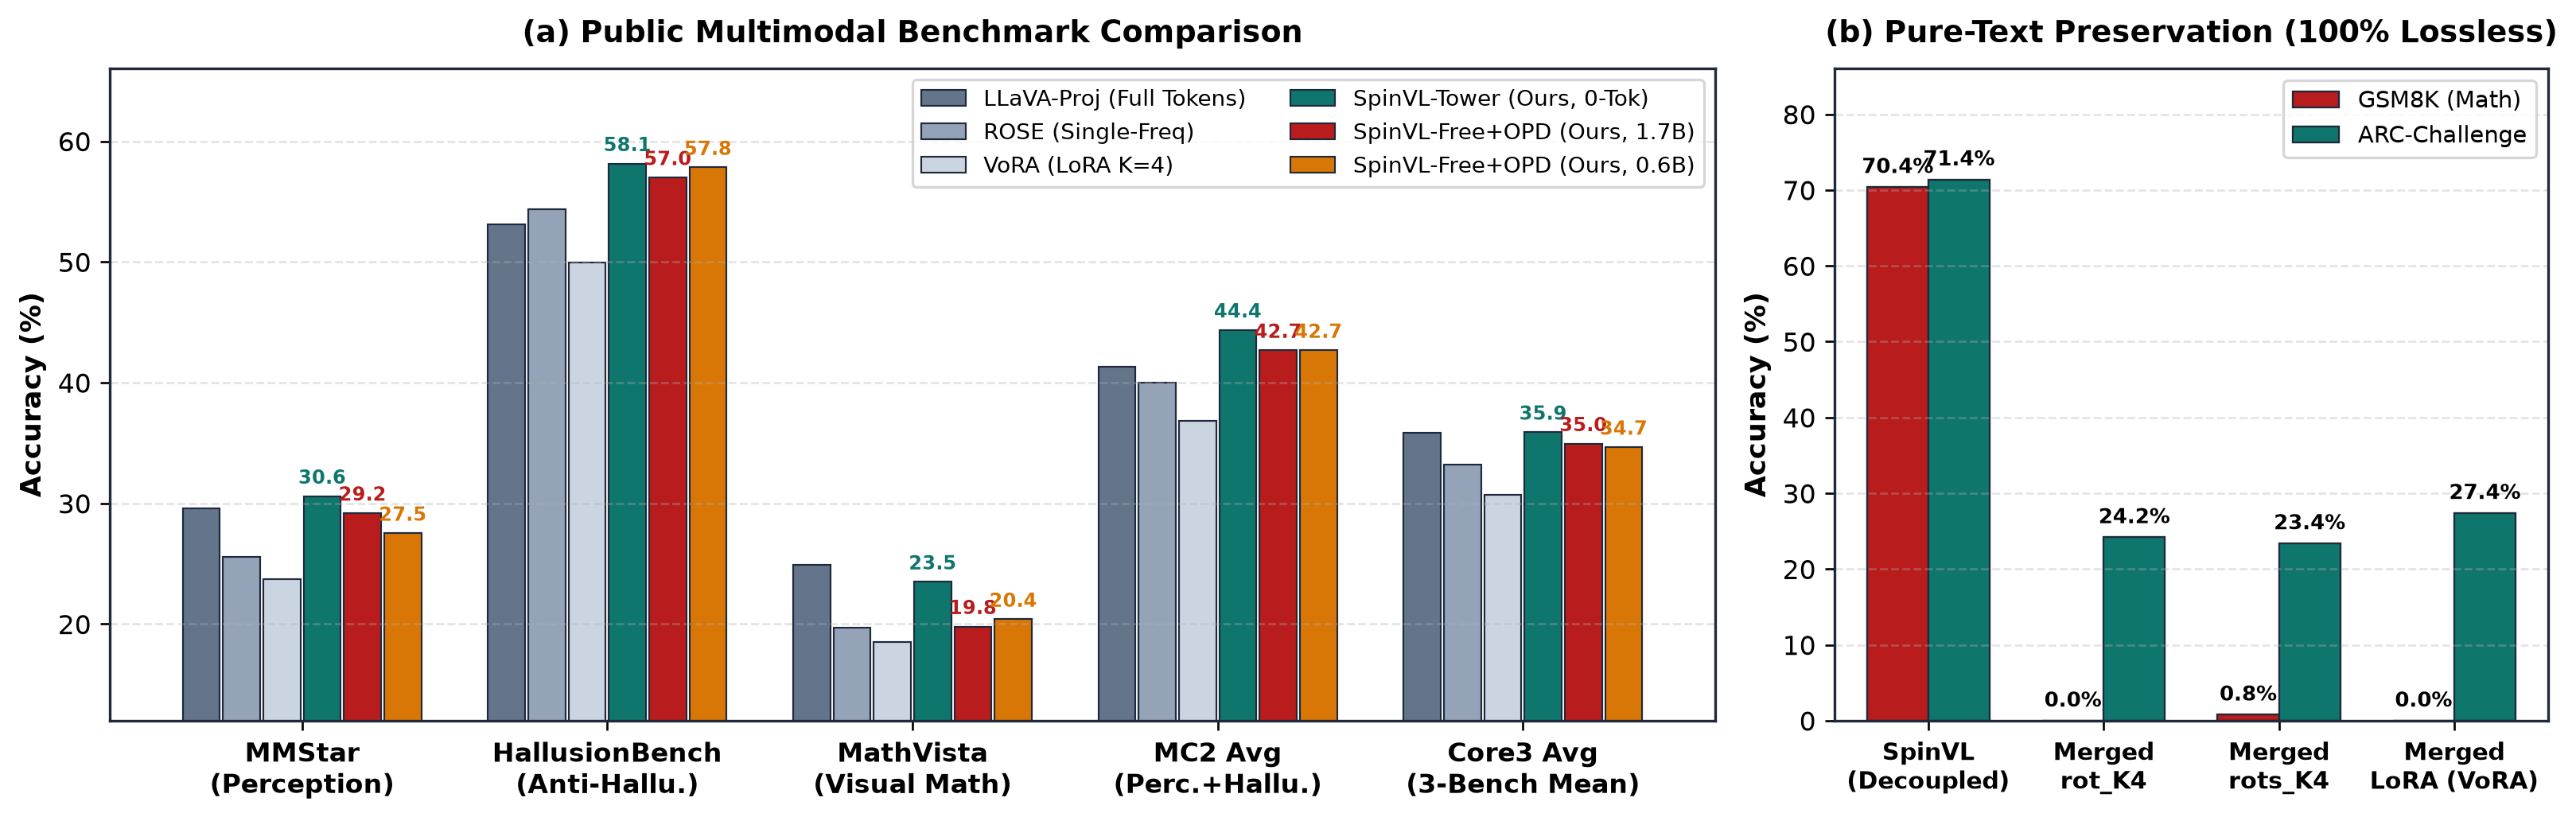
\includegraphics[width=\linewidth]{fig_main_results.png}
\caption{\textbf{Left:} per-benchmark accuracy of the main comparisons
($1.7$B student, identical training data and steps). \modelname{} leads on
perception (MMStar) and hallucination (HallusionBench) while keeping the
backbone free of visual tokens; the tower-free variant is competitive with the
full-token baseline at a quarter of its compute. \textbf{Right:} pure-text
retention. Only the decoupled pathway preserves GSM8K; merging the same vision
adapters into the text layers---LoRA, rotation, or rotation with scaling---and
collapsing the model.}
\label{fig:mainres}
\end{figure}

Tab.~\ref{tab:main} and Fig.~\ref{fig:mainres} summarise the comparison.
Three observations follow.

\emph{(i) Perception and hallucination improve without any visual token.}
\modelname-Tower with the hybrid generator reaches $30.60\%$ on MMStar and
$58.15\%$ on HallusionBench, against $29.60\%$ and $53.10\%$ for the
token-concatenation baseline. The MC2 aggregate rises from $41.35\%$ to
$44.37\%$, that is $+3.02$ points, while the backbone processes text of length
$T$ rather than $T+N$ in every one of its $28$ layers. HallusionBench is
particularly instructive: judging whether a small object is really present
requires attending to a specific region, which the $16$ spatial anchors of the
hybrid generator provide even though no visual token is ever placed in the
sequence.

\emph{(ii) Diagram reasoning catches up once the mixture is fixed.} The
multi-frequency generator with on-policy distillation reaches $23.50\%$ on
MathVista, close to the baseline's $24.90\%$, and brings Core3 to $35.90\%$
against $35.87\%$ for token concatenation. The gain comes from the banded
attention: low-frequency blocks summarise the figure, while high-frequency
blocks revisit small regions across consecutive reasoning steps, which is the
behaviour MathVista rewards.

\emph{(iii) Removing the encoder costs little.} With no external vision tower
at all, joint training plus distillation keeps MC2 at $42.68\%$---still above
the full-token baseline---and Core3 at $34.95\%$, i.e.\ $97.4\%$ of the
baseline's Core3 while using $74.2\%$ fewer FLOPs. The gap is concentrated in
MathVista and Geo3K, where a fixed-resolution cell grid loses thin geometric
strokes that the teacher encoder, with its learned tokenisation, retains.

\emph{(iv) Both tiers contribute, and each contribution is measured within a
fixed pipeline.} Holding the deep tier fixed at hybrid and comparing frontends
in the same arm, rotation with scaling beats rank-$16$ LoRA by $1.30$ points of
MC2 and $0.59$ of Core3. Holding the frontend fixed (external encoder) and
comparing deep generators, multi-frequency and hybrid rotation beat
single-frequency rotation by $0.75$ and $4.39$ points of MC2 respectively.
Composing both tiers with distillation yields the $44.37\%$ reported above, so
the gain is not attributable to a single component.

\subsection{Scaling Across Student Sizes and Seeds}
\label{sec:scaling}

\begin{table}[t]
\centering
\caption{\textbf{Cross-size behaviour and seed variance} (public benchmarks).
$0.6$B models are competitive with $1.7$B baselines on perception; $8$B
students do not benefit, since the frozen backbone is not the bottleneck.
Variation across three seeds is small relative to the gaps between methods.}
\label{tab:scale}
\footnotesize
\setlength{\tabcolsep}{3.0pt}
\begin{tabular}{@{}llcccccc@{}}
\toprule
Scale & Model & MMStar & Hallu. & MathV. & MC2 & Core3 & Avg6 \\
\midrule
$0.6$B & Tower (\texttt{hyb})          & 26.40 & 57.73 & 20.20 & 42.06 & 34.78 & 17.97 \\
$0.6$B & Free (CE)                    & 28.07 & 54.68 & 20.40 & 41.37 & 34.38 & 18.03 \\
$0.6$B & Free+OPD (base)              & 28.87 & 54.47 & 19.00 & 41.67 & 34.11 & 17.69 \\
$0.6$B & Free+OPD ($3$ seeds)         & 25.35$_{\pm2.21}$ & \textbf{57.69}$_{\pm0.10}$ & 18.73$_{\pm0.09}$ & \textbf{41.52}$_{\pm1.14}$ & \textbf{33.93}$_{\pm0.74}$ & \textbf{17.62}$_{\pm0.41}$ \\
\midrule
$1.7$B & Tower (\texttt{hyb}, $3$ seeds) & 26.56$_{\pm1.21}$ & 56.36$_{\pm0.85}$ & 18.97$_{\pm0.97}$ & 41.46$_{\pm0.62}$ & 33.96$_{\pm0.48}$ & 17.68$_{\pm0.35}$ \\
$1.7$B & Free+OPD ($3$ seeds)         & \textbf{26.11}$_{\pm2.62}$ & 56.11$_{\pm1.42}$ & \textbf{19.13}$_{\pm0.82}$ & 41.12$_{\pm1.10}$ & 33.79$_{\pm0.86}$ & 17.49$_{\pm0.24}$ \\
\midrule
$8$B   & Tower (\texttt{hyb})          & 25.67 & 54.15 & 19.90 & 39.91 & 33.24 & 17.30 \\
$8$B   & Free (\texttt{hyb})           & 24.80 & \textbf{56.99} & 19.20 & 40.90 & 33.66 & 17.50 \\
$8$B   & Free+OPD                     & \textbf{27.40} & 53.31 & 18.10 & 40.36 & 32.94 & 16.91 \\
\bottomrule
\end{tabular}
\end{table}

Tab.~\ref{tab:scale} reports the same pipelines with $0.6$B and $8$B students.
A $0.6$B tower-free model reaches $42.68\%$ MC2 and $18.05\%$ Avg6, matching or
exceeding the $1.7$B token-concatenation baseline on perception and
hallucination; the smallest student is therefore already sufficient for the
abilities this paradigm provides. Scaling to $8$B does not help, and in our
measurements slightly hurts: because the backbone is frozen and only the
rotation generators are trained, additional capacity in the LLM does not
translate into better visual steering, while a larger model makes optimisation
of the small adapter set harder at a fixed step budget. We see this as
evidence that the bottleneck is the interface, not the language model.

Repeating the two main configurations with three seeds gives standard
deviations of $0.35$--$2.62$ points, below the between-method differences we
report.

\subsection{Ablations}
\label{sec:abl}

\begin{table}[t]
\centering
\caption{\textbf{Frontend parameterisation.} Rows are grouped by training arm
because the four frontend modes were trained under two different rotation
initialisations; comparisons are made only within a group (see text). ``Val
CE'' and ``1st/Full'' are internal validation numbers on the base mixture; the
last column merges the frontend into the text layers and measures GSM8K.
Rotation with scaling is the only variant that is both accurate and safe to
merge-free.}
\label{tab:front}
\footnotesize
\setlength{\tabcolsep}{2.6pt}
\begin{tabular}{@{}llcccccc@{}}
\toprule
Frontend & Arm & Params & Val CE$\downarrow$ & 1st/Full & MC2 & Core3 & GSM8K \\
\midrule
none ($K{=}0$)     & rel & 0     & 5.237 & 24.0/16.0 & 35.92 & 31.15 & 70.4 \\
rot                & rel & 2.32M & 1.973 & 40.7/17.3 & \textbf{40.73} & \textbf{33.89} & \textbf{70.4} \\
full copy          & rel & 201M  & 1.745 & 43.3/20.0 & 38.82 & 32.08 & 0.0 \\
\midrule
LoRA ($r{=}16$)    & ce  & 3.74M & 1.532 & 44.7/18.7 & 36.84 & 30.73 & 0.0 \\
\textbf{rot+scale (\texttt{rots})} & ce & \textbf{2.40M} & 1.554 & 43.3/16.0 & \textbf{38.14} & \textbf{31.32} & \textbf{70.4} \\
\bottomrule
\end{tabular}
\end{table}

\paragraph{Frontend parameterisation (Sec.~\ref{sec:abl}).}
Tab.~\ref{tab:front} isolates the four ways of turning the first $K$ layers
into an encoder. Two groups were trained under different rotation
initialisations, so we compare inside each group. Within the first group, pure
rotation reaches $40.73\%$ MC2 with $2.32$M parameters, ahead of copying the
layers ($38.82\%$, $201$M) and of dropping the layers entirely
($35.92\%$): the frozen layers do the encoding work, and doing it with an
orthogonal transform is both cheaper and better than unfreezing copies. Within
the second group, rotation with channel scaling is ahead of rank-$16$ LoRA on
MC2 ($38.14$ vs.\ $36.84$), Core3 ($31.32$ vs.\ $30.73$) and Avg6, while
keeping GSM8K at $70.4\%$ against $0.0\%$ once the adapter is merged. The
margin over LoRA is thus smaller than the margin our full pipeline shows in
Tab.~\ref{tab:main}, and we attribute the difference to the deep tier and to
distillation rather than to the frontend alone. Finally, adding the deep
hybrid rotation and OPD to the same \texttt{rots} frontend lifts MC2 from
$38.14\%$ to $42.68\%$, i.e.\ the two tiers compose.

\paragraph{Depth of the built-in encoder.}
\begin{table}[t]
\centering
\caption{\textbf{Frontend depth} on the \emph{+open} mixture. Grounding gap
is the cross-entropy difference between shuffled and correctly paired images:
it measures how much the model actually uses the image.}
\label{tab:depth}
\footnotesize
\setlength{\tabcolsep}{4pt}
\begin{tabular}{@{}lcccccc@{}}
\toprule
$K$ & Params & CE$\downarrow$ & Gap$\uparrow$ & 1st$\uparrow$ & MC2 & Avg6 \\
\midrule
0 & 0      & 2.382 & 0.387 & 30.7 & 42.31 & 17.94 \\
2 & 1.20M  & 2.267 & 0.815 & 36.7 & 41.30 & 17.68 \\
\textbf{4} & \textbf{2.40M} & \textbf{2.248} & \textbf{1.070} & \textbf{37.3} & \textbf{42.68} & \textbf{18.02} \\
6 & 3.59M  & 2.272 & 0.978 & 38.0 & 41.94 & 17.66 \\
\bottomrule
\end{tabular}
\end{table}
Tab.~\ref{tab:depth} varies $K$. Grounding gap rises from $0.39$ at $K{=}0$ to
$1.07$ at $K{=}4$ and saturates afterwards, so four layers are enough to turn
textual attention into a usable image encoder; going deeper adds parameters
and cost without adding accuracy.

\paragraph{On-policy distillation and feature supervision.}
\begin{table}[t]
\centering
\caption{\textbf{Effect of Step~2.} Top: free-form generation with candidate
scoring disabled, so the model must produce the answer string itself.
Bottom: internal accuracy on the validation split.}
\label{tab:opd}
\footnotesize
\setlength{\tabcolsep}{4pt}
\begin{tabular}{@{}llccc@{}}
\toprule
Pair & Split & MMStar & Hallu. & MathV. \\
\midrule
$0.6$B Free & before & 14.53 & 23.55 & 9.70 \\
            & after  & \textbf{22.20} & \textbf{33.44} & \textbf{14.40} \\
\midrule
$1.7$B Free (base) & before & 14.07 & 24.40 & 8.30 \\
                   & after  & \textbf{18.13} & 22.92 & \textbf{9.30} \\
\midrule
$1.7$B Free ($28$k) & before & 25.33 & 0.11 & 12.20 \\
                    & after  & 25.07 & \textbf{1.26} & \textbf{16.30} \\
\bottomrule
\end{tabular}
\end{table}

Tab.~\ref{tab:opd} reports the effect of on-policy distillation when the model
must generate answers instead of scoring candidates. On the $0.6$B tower-free
model it adds $+7.67$ points on MMStar, $+9.89$ on HallusionBench and $+4.70$
on MathVista, and it raises end-of-sequence termination from $87\%$ to
$98\%$. The one regression we observe ($1.7$B, HallusionBench, base mixture)
comes with a shorter mean generation length, i.e.\ the model stops earlier
rather than answering differently; the same configuration recovers on the
\emph{+open} mixture, where HallusionBench free-form accuracy moves from
$0.11\%$ to $1.26\%$. We also verify that the frontend does not merely imitate
the teacher: switching off the feature term of Eq.~\eqref{eq:feat} during joint
training still yields $42.63\%$ MC2 and $18.13\%$ Avg6, within noise of the
supervised variant.

\subsection{Efficiency and Text Retention}
\label{sec:eff}

\begin{table}[t]
\centering
\caption{\textbf{Compute and latency} at increasing image resolution
($1.7$B, text query length $64$). Latency is measured with the GPU
exclusively occupied. At $4096$ patches \modelname{} needs $74.2\%$ fewer
FLOPs and is $19.5\%$ faster than token concatenation.}
\label{tab:eff}
\footnotesize
\setlength{\tabcolsep}{4pt}
\begin{tabular}{@{}rcccc@{}}
\toprule
Patches & \modelname{} & ROSE & LLaVA & Saving \\
 & (TFLOPs/ms) & (TFLOPs/ms) & (TFLOPs/ms) & FLOPs \\
\midrule
256  & 0.30/65.8  & 0.47/58.2  & 0.66/25.7  & $-54.8\%$ \\
576  & 0.45/66.6  & 0.86/57.8  & 1.27/25.6  & $-64.9\%$ \\
1024 & 0.67/69.8  & 1.45/63.8  & 2.18/33.7  & $-69.4\%$ \\
2304 & 1.37/80.4  & 3.40/86.0  & 5.07/66.9  & $-72.9\%$ \\
4096 & \textbf{2.54/99.4} & 6.82/126.1 & \textbf{9.85}/123.4 & $\mathbf{-74.2\%}$ \\
\bottomrule
\end{tabular}
\end{table}

\begin{figure}[t]
\centering
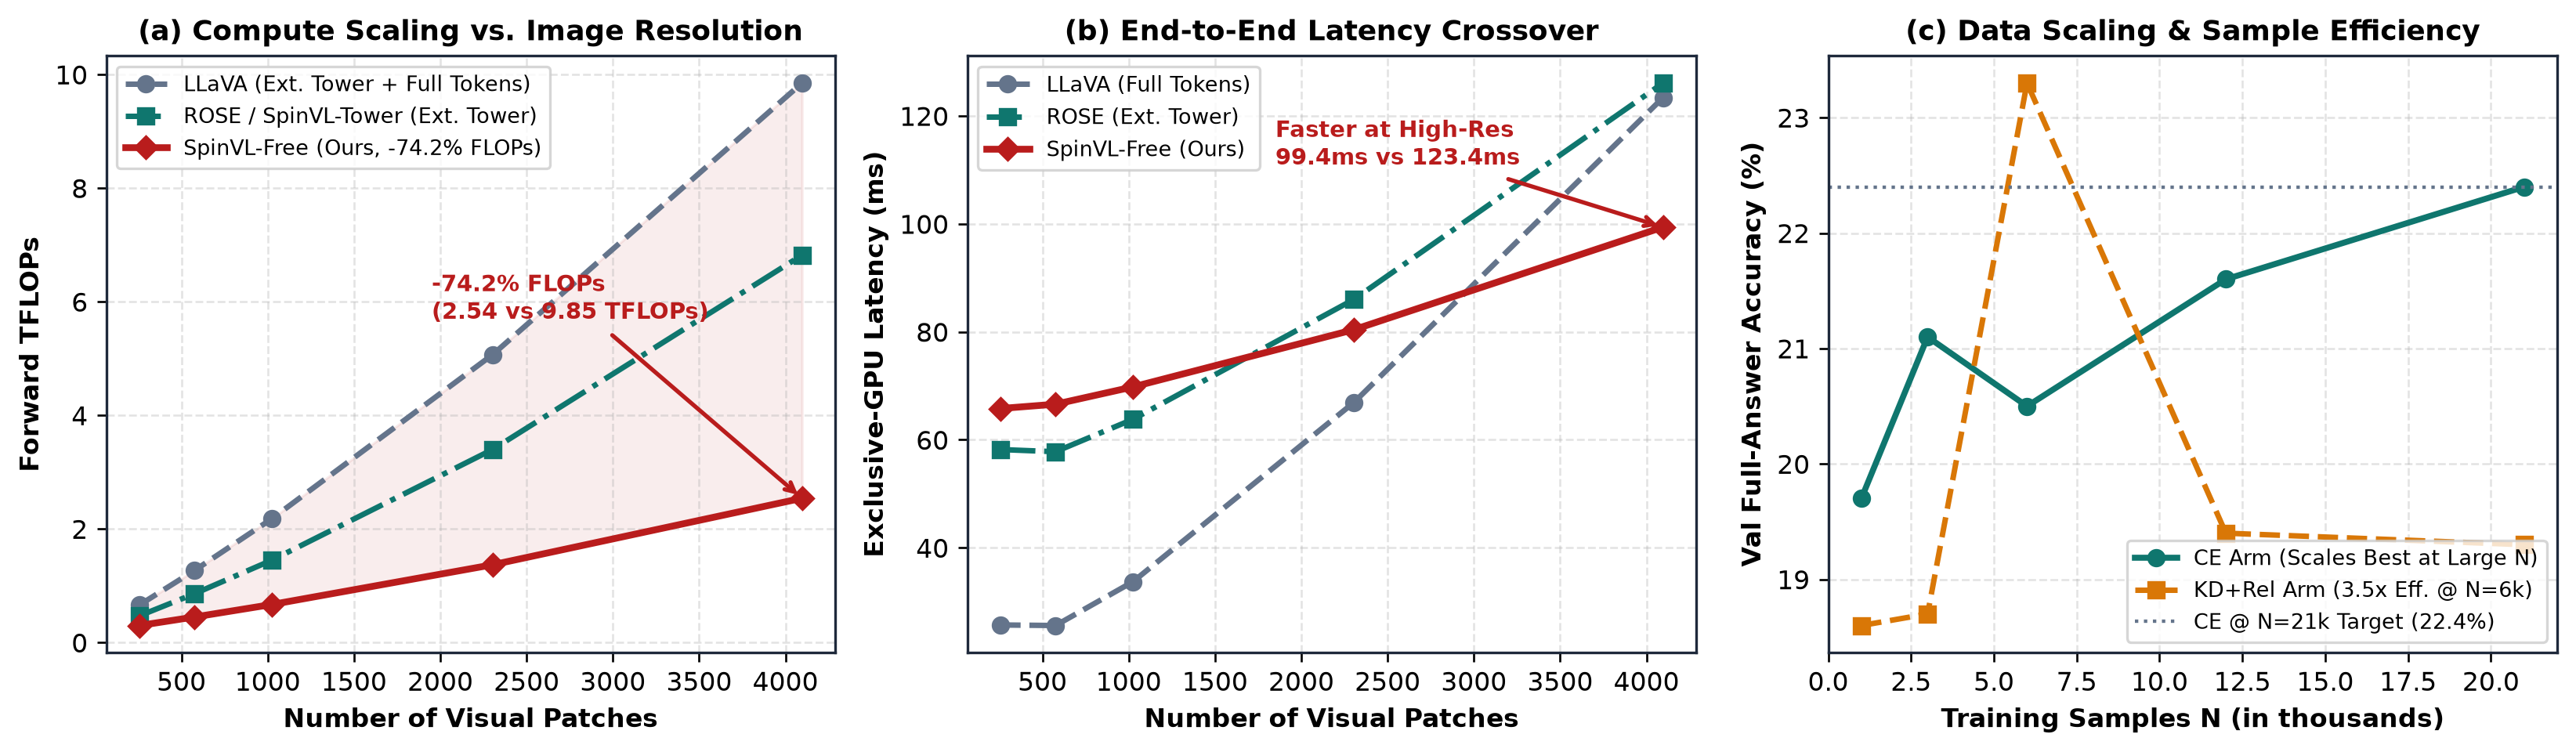
\includegraphics[width=\linewidth]{fig_efficiency.png}
\caption{\textbf{Efficiency and data scaling.} Top: forward cost and latency
versus visual patches; the advantage of discarding tokens grows with
resolution, and the crossover in latency appears beyond roughly $2$k patches.
Bottom: validation accuracy versus training-set size for the CE and
distillation arms; the distillation arm reaches at $6$k samples the accuracy
that the CE arm needs $21$k samples to attain.}
\label{fig:eff}
\end{figure}

Tab.~\ref{tab:eff} and Fig.~\ref{fig:eff} quantify the trade-off. The saving
grows with resolution because the baseline pays $O((T+N)^2)$ in every layer
while \modelname{} pays $O(N^2)$ once for $K$ layers. Below roughly $2$k
patches the baseline is still faster in wall-clock terms on our hardware, since
the frontend's bidirectional pass over all patches is not free; beyond that the
ordering reverses and the gap widens.

Text retention is reported in Fig.~\ref{fig:mainres} (right). The decoupled
pathway keeps GSM8K at $70.4\%$ and ARC-C at $71.4\%$, identical to the
unmodified LLM. Merging the frontend into the text layers---whether as LoRA,
pure rotation, or rotation with scaling---drops GSM8K to $0.0\%$, $0.0\%$ and
$0.8\%$ respectively. This is the clearest argument for keeping vision
adapters context-gated instead of permanently fused.

\subsection{Where the Paradigm Stops: A Controlled Boundary Study}
\label{sec:boundary}

\begin{table}[t]
\centering
\caption{\textbf{Boundary study.} Adding $8{,}334$ open-ended document/chart
questions and $2{,}101$ geometry problems to the training mixture
($21$k$\to$$28$k). Geometry doubles for \modelname{}, whereas character-level
chart reading and scene text stay flat for both methods: the residual gap is
architectural, not a data artefact.}
\label{tab:boundary}
\footnotesize
\setlength{\tabcolsep}{4pt}
\begin{tabular}{@{}llccc@{}}
\toprule
Mixture & Model & ChartQA & OCRBench & Geo3K \\
\midrule
base ($21$k)      & LLaVA-Proj & \textbf{10.40} & \textbf{1.60} & \textbf{6.49} \\
base ($21$k)      & \modelname-Tower & 1.08 & 0.00 & 1.83 \\
\midrule
+open ($28$k)     & LLaVA-Proj & \textbf{10.32} & \textbf{1.10} & 5.49 \\
+open ($28$k)     & \modelname-Tower & 1.24 & 0.00 & \textbf{3.83} \\
\bottomrule
\end{tabular}
\end{table}

Our benchmarks mix two very different demands. Perception, hallucination and
diagram reasoning ask \emph{what is in the image}; chart reading and OCR ask
the model to \emph{copy a string exactly}. To separate the two we first audited
the base mixture and found that it contains no open-ended chart item and no
scene-text item at all: the chart-like portion is entirely multiple choice.
That makes the low ChartQA and OCRBench numbers in Tab.~\ref{tab:main}
uninformative on their own, since no model in the comparison had seen the task
format.

We therefore rebuilt the mixture to include the missing formats and retrained
both the token-concatenation baseline and \modelname{} on it
(Tab.~\ref{tab:boundary}). Two results are decisive. First, the baseline's
ChartQA accuracy does not move ($10.40\%\to10.32\%$) and its OCRBench accuracy
falls ($1.60\%\to1.10\%$), even though $6{,}500$ document and chart questions
were added: exact copying is not a data problem for the baseline, it is a
capability it already has and the added data does not improve. Second,
\modelname{}'s geometry accuracy doubles ($1.83\%\to3.83\%$), so the added data
is being used where the architecture supports the task.

We read this as a statement about the operating envelope. Operator-level
modulation compresses the image into a small set of rotation parameters; it
can decide presence, count, layout, and can re-consult regions through
anchors, but it cannot maintain a per-character key-value memory. Copying a
five-digit axis label therefore fails for reasons that are structural rather
than statistical. We regard the honest statement of this boundary as a
contribution: it tells practitioners which abilities to expect from zero-token
injection, and it identifies dense transcription as the case where a small
number of retained visual tokens is likely necessary. All remaining
benchmarks in this paper---perception, hallucination, diagram and geometry
reasoning---fall inside the envelope.

\section{Limitations and Conclusion}
\label{sec:conclusion}

\paragraph{Limitations.}
We state four limits explicitly, because they define the regime in which the
claims hold.

\emph{Dense transcription remains out of reach.} As shown in
Sec.~\ref{sec:boundary}, exact character copying (chart axis labels, receipts,
handwritten formulae) does not follow from operator-level modulation, and the
data study we ran---retraining a token-concatenation baseline on identical
data---indicates that the gap is architectural rather than a data artefact. A
practical extension is to retain a small number of pooled visual tokens for
this class of queries only; we deliberately do not include such a variant here,
because it would break the zero-token property that the paper is about.

\emph{The backbone is never adapted.} Keeping the LLM frozen is what buys
bit-exact text retention and cheap training, but it also caps the achievable
accuracy: a $8$B student is no better than a $0.6$B one in our measurements,
which suggests that the adapter interface, not the language capacity, is the
bottleneck. Allowing even a low-rank update of the backbone would likely raise
the ceiling, at the cost of the lossless property.

\emph{Training scale is modest.} Our mixtures contain $21$k and $28$k
short-answer items and a single teacher; we have not studied web-scale
pretraining of the rotation generators. Sample-efficiency curves
(Fig.~\ref{fig:eff}) indicate that distillation makes small mixtures viable,
but we cannot claim behaviour at the scale used by industrial VLMs.

\emph{Two-phase inference.} The tower-free variant runs a bidirectional pass
over patches and then a causal pass over text, which prevents a single fused
kernel from covering both phases. Our latency numbers include both phases on
one GPU, but a production deployment would need a fused implementation to
realise the full benefit.

\paragraph{Conclusion.}
We asked whether a frozen text LLM can be given vision without an external
encoder and without paying for visual tokens in its backbone. \modelname{}
answers with a dual-tier orthogonal rotation architecture---static rotation
with channel scaling in the first $K$ layers to encode the image, then dynamic
block-diagonal rotations generated by multi-frequency or spatial-anchor
queries in the remaining frozen layers---followed by on-policy distillation
over the student's own rollouts. Under identical data, steps and base models,
the resulting models exceed a token-concatenation baseline on visual
perception and hallucination resistance ($44.37$ vs.\ $41.35$ MC2), match it on
the average of perception, hallucination and diagram reasoning ($35.90$ vs.\
$35.87$), beat both single-frequency rotation and LoRA-based built-in encoders
by clear margins, reduce FLOPs by $74.2\%$ and latency by $19.5\%$ at high
resolution, and leave pure-text ability untouched at $70.4\%$ GSM8K and
$71.4\%$ ARC-C. The same recipe transfers to a $0.6$B student. Equally
important, we delimit what the paradigm does not do: operator-level modulation
buys semantic perception, layout reasoning and hallucination resistance, but
not dense character transcription, which we trace to the absence of
per-position key-value addressing. We hope both halves of that statement are
useful---the positive one for building lightweight multimodal models from
frozen LLMs, and the boundary one for deciding when a few visual tokens are
worth their cost.
{\small
\bibliographystyle{plainnat}
\bibliography{references}
}

\end{document}
